\documentclass[11pt]{jsarticle}

\usepackage[top=30mm, bottom=36mm, left=28mm, right=28mm]{geometry}
\usepackage[dvipdfmx]{graphicx}
\usepackage{url}
\usepackage{amssymb}

\usepackage{mytitle}

\title{3. 画像のループバック}
\author{201720690 小松 弘人}
\date{2017/06/12}

\makeatletter
\def\mojiparline#1{
    \newcounter{mpl}
    \setcounter{mpl}{#1}
    \@tempdima=\linewidth
    \advance\@tempdima by-\value{mpl}zw
    \addtocounter{mpl}{-1}
    \divide\@tempdima by \value{mpl}
    \advance\kanjiskip by\@tempdima
    \advance\parindent by\@tempdima
}
\makeatother
\def\linesparpage#1{
    \baselineskip=\textheight
    \divide\baselineskip by #1
}

\begin{document}
\maketitle
\subsection*{演習目的}
本演習の進め方を理解する。
FIFOの基礎を実践しながら理解する。

\subsection*{演習概要}
ZedBoardでXillinuxを起動し、その上でARMからFPGAに画像データを
送るプログラムを実行し、結果画像を確認する。
そのために、まずはVivadoで画像をループバックさせるための回路を記述する。
次に、ブートに必要なファイルをSDカードに入れ、
ZedBoard上でXillinuxを起動する。
最後に、結果が正しいかどうかを確認する。

\subsection*{事前準備}
\subsubsection*{Vivadoでxillydemoプロジェクトを作成する (Windows)}
チュートリアルのページから、xillinuxリポジトリをダウンロードしておくこと。
Vivadoを起動し、Tools→Run Tcl Script...から
verilog/xillydemo-vivado.tclを実行する。
しばらく待つと、xillydemoプロジェクトが開く。
このプロジェクトのxillydemo.vにフィルタ回路などを追加する。
実機で試す際には、Generate Bitstreamまで実行すること。

\subsubsection*{Xillinuxのブート用SDカードを作成する (Linux版)}
詳細は``Getting started with Xillinux for Zynq-7000 EPP''参照。
公式ホームページ (\url{http://xillybus.com/xillinux}) から、
SDカードイメージをダウンロードする (図\ref{img:xillinux})。
なお、前述のドキュメントはその下のリンクからアクセスできる。

\begin{figure}[ht]
	\centering
	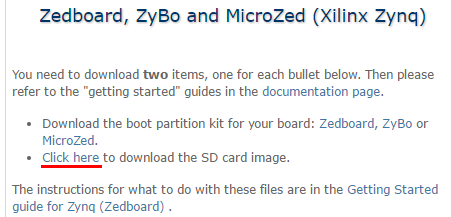
\includegraphics[width=0.5\linewidth]{img/xillinux.PNG}
	\caption{Xillinux: A Linux distribution for Zedboard, ZyBo, MicroZed and SocKit}
	\label{img:xillinux}
\end{figure}

\vspace{-0.5cm}

xillinux-1.3.img.gzを解凍し、xillinux-1.3.imgを得る。
それを\verb|dd|でSDカードに書き込む。
書き込みが終わったら、SDカードの第1パーティションに
xillinuxリポジトリの中にあるbootfiles内の2つのファイルをコピーする。
同様に、xillydemoプロジェクトの中
(verilog/vivado/xillydemo.runs/impl\_1) にあるxillydemo.bitを
コピーする。

\subsubsection*{Xillinuxの環境設定・事前準備 (Xillinux)}
\verb|startx|でGUIを起動できる。
演習に用いるプログラムは、GUIなしでも実行できるが、
コンソールのデフォルトキーボードレイアウトは
英字配列であるため、不便である。
したがって、GUIを起動することをおすすめする。

\begin{itemize}
	\item
		キーボードの設定: System Settings→Keyboard Layoutから
		Japaneseを追加
	\item
		IPアドレスの設定: System Settings→Network→Wired→Options...から
		IPv4アドレスを設定
	\item
		apt-getでgit, g++, openssh-serverのインストール
	\item
		passwdでパスワードを設定
\end{itemize}

\subsection*{演習内容}
\subsubsection*{Xillinuxの演習 (Windows)}
Vivadoでxillydemoプロジェクトを開く。
Add sourcesからAdd or create design sourcesを選択し、Nextをクリック。
Create Fileを選択し、File typeはそのまま、File nameはloopback、
File locationはuserfiles/verilogとし、OKをクリック。
元のダイアログに戻ったらFinishをクリック。
モジュールの入出力ピンの指定が求められるため、
表\ref{tbl:inout}のように設定する。
入力が終わったらOKを押して、ファイルを作成する。

\begin{table}[ht]% Table 1
	\caption{In/out ports.}
	\label{tbl:inout}
	\begin{center}
		\begin{tabular}{ccccc}
			\hline
			Portname & Direction & Bus & MSB & LSB \\
			\hline \hline
			clk & input &   & - & - \\
			srst & input &   & - & - \\
			din & input & \checkmark & 31 & 0 \\
			wr\_en & input &   & - & - \\
			rd\_en & input &   & - & - \\
			dout & output & \checkmark & 31 & 0 \\
			full & output &   & - & - \\
			empty & output &   & - & - \\
			\hline
		\end{tabular}%
	\end{center}
\end{table}

その後、\verb|wrapper.v|を編集し、\verb|loopback|を
\verb|line_buf|の後に追加する。
このとき、\verb|dco|を\verb|din|に接続し、それ以外は無視する。
さらに、\verb|loopback.v|を編集する。
\verb|loopback|モジュールの回路図を図\ref{img:loopback}に示す。
\verb|ce|は、各レジスタのクロックイネーブル信号である。
まず、シフトレジスタを\verb|din|や\verb|wr_en|に追加する。
また、\verb|fifo_fwft_32x16|を追加し、接続する。
編集したら、Generate Bitstreamを実行する。
その後、xillydemo.bitをSDカードにコピーし、ZedBoardを起動する。

\begin{figure}[ht]
	\centering
	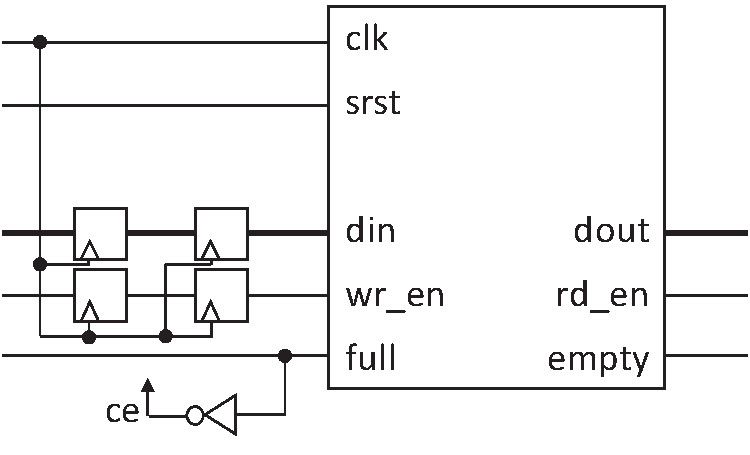
\includegraphics[width=0.5\linewidth]{img/loopback.pdf}
	\caption{loopbackモジュールのブロック図}
	\label{img:loopback}
\end{figure}

\vspace{-0.5cm}

\subsubsection*{演習用プログラムの実行 (Xillinux)}
Xillinuxに、チュートリアルのページから、
softwareリポジトリをダウンロードし、展開しておくこと。
展開したディレクトリでmakeを実行すると、
\verb|bin/send_bmp|ができる。
下記のように実行する。

\begin{center}
	\verb|bin/send_bmp src.bmp dst.bmp|
\end{center}

\subsubsection*{結果画像の確認}
出力画像が入力画像をグレースケールにした画像となることを確認する。
Xillinuxのディスプレイは各色4bitであるため、
正しく画像の比較ができない。
そこで、\verb|ssh|などで別コンピュータに移動し、
確認することを薦める。

\subsubsection*{Verilogの最低限の文法}
調べたほうが詳しく分かりやすく出るが、
Verilogの最低限の文法を記載していく。\\
\begin{verbatim}
// コメント
/* 複数行コメント */

/* 変数宣言 */
wire wa; // 1bitの配線を宣言
wire [7:0] wb; // 8bitの配線を宣言
reg ra; // 1bitのレジスタを宣言
reg [7:0] rb = 8'h00; // 8bitのレジスタを宣言し初期化
assign wa = ra; // 継続的代入

/* 数字リテラル */
2'b10 // 2進数表記 2 (2bit)
8'd10 // 10進数表記 10 (8bit)
8'h10 // 16進数表記 16 (8bit)

/* 演算子 */
wa + wb; // 加算
wa - wb; // 減算
wa * wb; // 乗算
wa >> 1; // 論理右シフト
wa << 1; // 論理左シフト
wa >>> 1; // 算術右シフト
wb & 8'h0f; // AND演算
wb | 8'h0f; // OR演算
wb ^ 8'h0f; // XOR演算
~wa // 否定
wb == rb // 比較 (等号)
wb != rb // 比較 (不等号)
wb < rb // 比較
wb >= rb // 比較

/* 信号の連結 */
{8'h00, rb} // 16bit

/* 信号の特定bitの抽出 */
wb[3:0] // 下位4bit

/* 組み合わせ回路の記述 */
always@(posedge clk) // clkの立ち上がりで実行する
begin
    ra = wa; // ブロッキング代入
    rb <= wb; // ノンブロッキング代入
end
\end{verbatim}

\end{document}
